\documentclass[tikz,border=14pt]{standalone}
\usepackage{amsmath}

\definecolor{pinkfill}{HTML}{FFF0F6}
\definecolor{pinkedge}{HTML}{C2255C}
\definecolor{ink}{HTML}{343A40}

\begin{document}
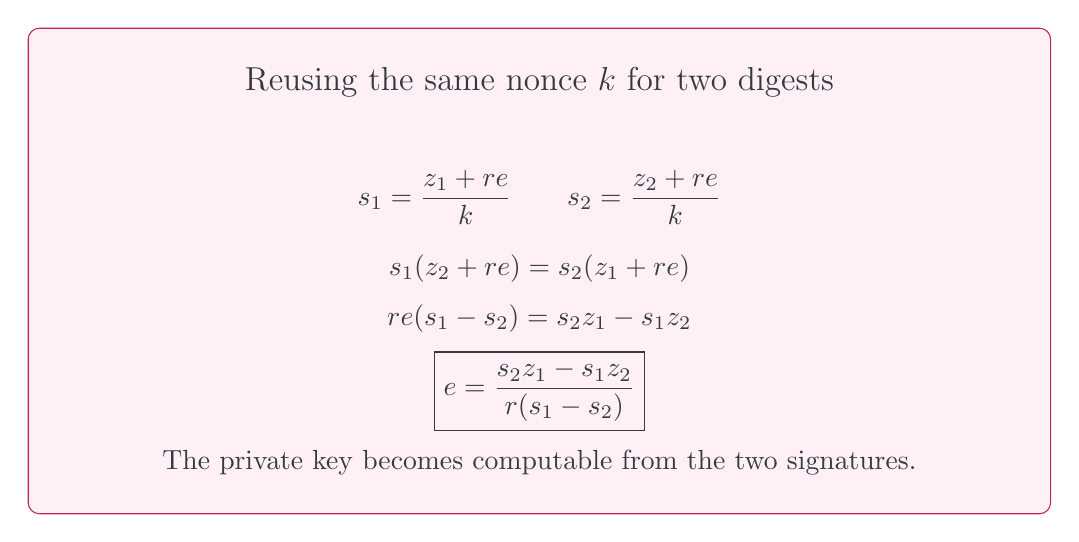
\begin{tikzpicture}
  \node[draw=pinkedge, fill=pinkfill, rounded corners=4pt, inner sep=14pt, text=ink] {
    \begin{minipage}{12cm}
      \centering
      {\large Reusing the same nonce $k$ for two digests}\par\medskip
      \[
        s_1=\frac{z_1+re}{k}
        \qquad
        s_2=\frac{z_2+re}{k}
      \]
      \[
        s_1(z_2+re)=s_2(z_1+re)
      \]
      \[
        re(s_1-s_2)=s_2z_1-s_1z_2
      \]
      \[
        \boxed{e=\frac{s_2z_1-s_1z_2}{r(s_1-s_2)}}
      \]
      The private key becomes computable from the two signatures.
    \end{minipage}
  };
\end{tikzpicture}
\end{document}
